% =====================================================================
%  Introduction to Deep Learning — Class 28
%  Topic (course plan): Recurrent Neural Network
%  Subtopic (course plan): LSTM and Gated RNNs
%  Sources (course plan): Jurafsky & Martin Ch. 13 (Ch. 14 in the
%    August 2026 draft), Goodfellow Ch. 10
%
%  Class 27 treated the recurrent cell g as a black box.  This class
%  opens it: why the simple cell forgets — the same product of Jacobians
%  Class 26 derived, seen through the eigenvalues of Class 13 — and what
%  a gate changes.  The object is the cell: what happens between h_{t-1}
%  and h_t.
%
%  Order: the problem (long-term dependencies, the power method, the
%  gradient measured); the ancestors of the gate (skip connections,
%  leaky units, echo state networks); the LSTM and the GRU; the
%  optimisation fixes (clipping, the information-flow regulariser);
%  where the gate leads (explicit memory).
%
%  A variant: every figure is the published one, cropped from the
%  book PDF by crop_figures.py and cited on the slide.  See _shared/PLAN_Classes26_27_28_29.md.
%
%  Compile:  xelatex main.tex   (run twice)
% =====================================================================
\documentclass[aspectratio=169, 11pt]{beamer}

\usetheme{metropoliscustom}

\usepackage{graphicx}
\DeclareGraphicsExtensions{.pdf,.png,.jpg}
\graphicspath{{figs_official/}{Class28_LSTM_Gated_RNNs/A_Textbook_Figures/figs_official/}}
\usepackage{amsmath, amssymb}
\usepackage{bm}
\usepackage{tikz}
\usetikzlibrary{arrows.meta, positioning, calc, decorations.pathreplacing,
                shapes.geometric, fit, backgrounds}
\tcbuselibrary{skins}

\definecolor{shc}{HTML}{341651}
\definecolor{tealc}{HTML}{1C7293}
\definecolor{dpc}{HTML}{800000}
\definecolor{accc}{HTML}{B8860B}

% ---- theorem environments -------------------------------------------
\setbeamertemplate{theorems}[numbered]
\usepackage{remreset}
\makeatletter\@removefromreset{theorem}{section}\makeatother
\renewcommand{\thetheorem}{\arabic{theorem}}
\newtheorem{lemmax}[theorem]{Lemma}
\newtheorem{propx}[theorem]{Proposition}
\newtheorem{corx}[theorem]{Corollary}
\newtheorem{defx}[theorem]{Definition}
\newtheorem{thmx}[theorem]{Theorem}

\newcommand{\bridge}[1]{%
  {\scriptsize\itshape\color{mcMuted} #1\par}\vspace{0.35em}}

\newcommand{\srcline}[1]{%
  \par\vspace{0.25em}%
  {\scriptsize\color{mcMuted}\hfill #1\par}}

\newcommand{\figsource}[1]{{\scriptsize\color{mcMuted} #1}}
\newcommand{\figcap}[2][0.90]{%
  \begin{center}\begin{minipage}{#1\textwidth}\centering
    {\scriptsize\color{mcMuted} #2}
  \end{minipage}\end{center}}

% =====================================================================
\title{Recurrent Neural Networks}
\subtitle{LSTM and Gated RNNs}
\author{Introduction to Deep Learning \ \textperiodcentered\ Class 28}
\institute{}
\date{}

\footleft{Introduction to Deep Learning}
\footright{LSTM and Gated RNNs}
\titlelogos{}

\begin{document}

\maketitle

\begin{frame}{Outline}
  \tableofcontents
\end{frame}

% =====================================================================
\section{Why a Simple Cell Forgets}
% =====================================================================

\begin{frame}{Opening the cell}
  \bridge{Class 27 used the recurrent cell $g$ as a black box. Today the
  box is opened: why $\mathbf{h}_t = g(\mathbf{U}\mathbf{h}_{t-1} + \mathbf{W}\mathbf{x}_t)$
  cannot hold a fact for long, and what a gate changes.}
  \vspace{-0.1em}
  {\footnotesize
  \begin{itemize}\itemsep0.28em
    \item \emph{The flights the airline was canceling \alert{were} full.}
          To choose \emph{were}, the model must carry the plural
          \emph{flights} across \emph{airline was}, which argues for the
          singular
    \item The hidden state has two jobs at once: serve the current
          decision, and carry what future decisions will need
    \item And the gradient that would teach it the second job passes
          through as many multiplications as there are steps between
          cause and effect
  \end{itemize}}
  \vspace{0.05em}
  \begin{redhighlight}
    Both problems have the same root: the state is overwritten at every
    step by the same matrix. A gate lets the network decide, at each
    step, what to overwrite.
  \end{redhighlight}
  \srcline{Jurafsky \& Martin (2026), \S14.5, example (14.19); Goodfellow et al.\ (2016), \S10.7.}
\end{frame}

\begin{frame}{Notation for today}
  \vspace{0.2em}
  {\footnotesize
  \renewcommand{\arraystretch}{1.28}
  \begin{columns}[T, onlytextwidth]
    \begin{column}{0.49\textwidth}
      \begin{tabular}{@{}l@{\hspace{1.3em}}l@{}}
        $\mathbf{h}_t$, $\mathbf{c}_t$ & hidden state and cell (context) state\\
        $\mathbf{f}_t, \mathbf{i}_t, \mathbf{o}_t$ & forget, add (input) and output gates\\
        $\mathbf{g}_t$ & the candidate written into the cell\\
        $\mathbf{u}_t, \mathbf{r}_t$ & the GRU's update and reset gates\\
      \end{tabular}
    \end{column}
    \begin{column}{0.49\textwidth}
      \begin{tabular}{@{}l@{\hspace{1.3em}}l@{}}
        $\odot$ & element-wise product\\
        $\sigma$ & the logistic sigmoid\\
        $\lambda_i$ & eigenvalues of $\mathbf{U}$, as in Class 13\\
        $\mathbf{J}_t$ & $\partial\mathbf{h}_t/\partial\mathbf{h}_{t-1}$, the step Jacobian\\
      \end{tabular}
    \end{column}
  \end{columns}}
  \vspace{0.45em}

  \begin{itemize}\itemsep0.22em
    \item Jurafsky's letters throughout: $\mathbf{U}$ recurrent, $\mathbf{W}$
          input, each gate with its own pair. Goodfellow swaps
          $\mathbf{U}$ and $\mathbf{W}$, writes the cell $\mathbf{s}$, the
          input gate $\mathbf{g}$ and the output gate $\mathbf{q}$
    \item Every equation from Goodfellow below is transcribed into
          these letters, with his number beside it
  \end{itemize}
  \srcline{Jurafsky \& Martin (2026), Eqs.~14.20--14.27; Goodfellow et al.\ (2016), Eqs.~10.40--10.47.}
\end{frame}

\begin{frame}{The linear case: a power iteration}
  \vspace{-0.45em}
  \begin{thmx}[Vanishing and exploding, without a nonlinearity]\label{th:power}
    \small
    For the recurrence $\mathbf{h}_t = \mathbf{U}\mathbf{h}_{t-1}$ with
    $\mathbf{U} = \mathbf{Q}\bm{\Lambda}\mathbf{Q}^{\mathsf T}$ orthogonally diagonalisable,
    \[
      \mathbf{h}_t = \mathbf{U}^t\mathbf{h}_0 = \mathbf{Q}\bm{\Lambda}^t\mathbf{Q}^{\mathsf T}\mathbf{h}_0 ,
    \]
    so the component of $\mathbf{h}_0$ along eigenvector $i$ is multiplied
    by $\lambda_i^t$: geometric decay if $|\lambda_i| < 1$, explosion if
    $|\lambda_i| > 1$; only the largest survives.
  \end{thmx}
  \vspace{-0.15em}
  {\footnotesize
  \begin{itemize}\itemsep0.12em
    \item \focus{1}{Proof. $(\mathbf{Q}\bm{\Lambda}\mathbf{Q}^{\mathsf T})^t
          = \mathbf{Q}\bm{\Lambda}^t\mathbf{Q}^{\mathsf T}$ since
          $\mathbf{Q}^{\mathsf T}\mathbf{Q} = \mathbf{I}$, and $\bm{\Lambda}^t$ has
          entries $\lambda_i^t$. \hfill $\square$}
    \item \focus{2}{The power method of Class 13, on the recurrent
          matrix instead of the Hessian. A feedforward net multiplies
          \emph{different} matrices, which can be scaled to compensate; a
          recurrent net multiplies the \emph{same} one.}
  \end{itemize}}
  \vspace{-0.3em}
  \srcline{Goodfellow et al.\ (2016), \S10.7, Eqs.~10.36--10.39; Class 13.}
\end{frame}

\begin{frame}{The composition, drawn}
  \begin{center}
    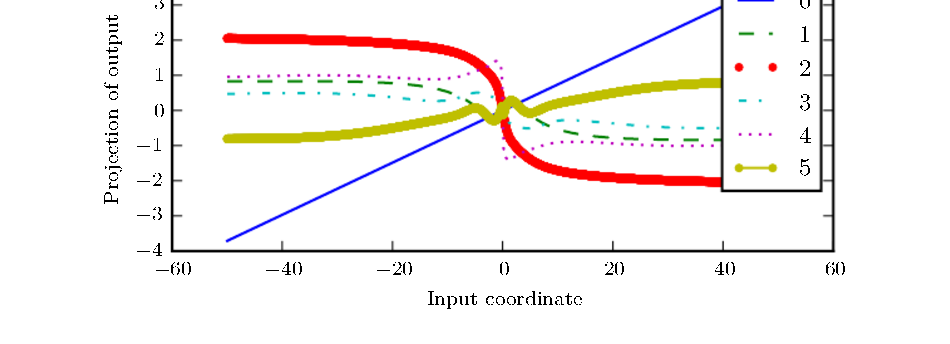
\includegraphics[width=0.80\linewidth]{G10_15}
  \end{center}
  \vspace{-0.5em}
  {\tiny\color{mcMuted}
  A linear--tanh layer composed many times: a linear projection of a
  $100$-dimensional hidden state onto one axis, plotted against the
  initial state's coordinate along a random direction. Most of the
  function has a tiny derivative, a few places a very large one, with
  many alternations between increasing and decreasing --- the cliffs
  the recurrent loss inherits.
  \hfill Goodfellow et al.\ (2016), Fig.~10.15.\par}
\end{frame}

\begin{frame}{With the nonlinearity: a bound on the gradient}
  \vspace{-0.45em}
  \begin{propx}[Sufficient condition for vanishing]\label{th:bound}
    \small
    For $\mathbf{h}_t = g(\mathbf{U}\mathbf{h}_{t-1} + \mathbf{W}\mathbf{x}_t)$ with
    $|g'| \leq \gamma$ everywhere ($\gamma = 1$ for $\tanh$, $\tfrac14$ for
    the sigmoid),
    \[
      \Big\| \frac{\partial\mathbf{h}_t}{\partial\mathbf{h}_k} \Big\|
      = \Big\| \prod_{s=k+1}^{t} \mathbf{J}_s \Big\|
      \leq \big( \gamma\,\|\mathbf{U}\| \big)^{t-k},
    \]
    so if $\|\mathbf{U}\| < 1/\gamma$ the gradient from $t$ back to $k$
    vanishes geometrically in the lag.
  \end{propx}
  \vspace{-0.15em}
  {\footnotesize
  \begin{itemize}\itemsep0.12em
    \item \focus{1}{Proof. $\mathbf{J}_s = \mathrm{diag}(g')\,\mathbf{U}$ by the
          chain rule of Class 26, so $\|\mathbf{J}_s\| \leq \gamma\|\mathbf{U}\|$;
          the norm of a product is at most the product of the norms.
          \hfill $\square$}
    \item \focus{2}{Sufficient, not necessary: it says when the gradient
          \emph{must} vanish. Either way a distant cause gets an
          exponentially smaller gradient than a recent one, so the
          recent ones win.}
  \end{itemize}}
  \vspace{-0.3em}
  \srcline{Pascanu, Mikolov \& Bengio (2013); Goodfellow et al.\ (2016), \S10.7; Bengio et al.\ (1994).}
\end{frame}


% =====================================================================
\section{Paths Through Time}
% =====================================================================

\begin{frame}{Three ways to a path the gradient survives}
  \vspace{0.05em}
  {\scriptsize
  \renewcommand{\arraystretch}{1.34}
  \begin{tabular}{@{}l@{\hspace{1.1em}}l@{\hspace{1.1em}}l@{}}
    \textbf{Idea} & \textbf{Mechanism} & \textbf{Cost}\\
    skip connections & an edge from $t - d$ to $t$; decay in $\tau/d$ & $d$ fixed and integer\\
    leaky units & a linear self-connection, weight $\alpha \approx 1$ & one time scale per unit\\
    removing connections & some units updated every $d$ steps & groups and rates by hand\\
    \alert{gates} & a self-connection weighted \alert{by the input} & more parameters; this class\\
  \end{tabular}}
  \vspace{0.3em}

  \begin{itemize}\itemsep0.2em
    \item All four build a path along which the product of derivatives
          stays near one, so a fact can reach the present from far back
    \item Echo state networks give up instead: fix $\mathbf{U}$ at a
          chosen spectral radius (near, or above, one, with $\tanh$ to
          bound it) and learn only the output weights, a convex problem
  \end{itemize}
  \srcline{Goodfellow et al.\ (2016), \S10.8--10.9; Lin et al.\ (1996); Mozer (1992); Jaeger \& Haas (2004).}
\end{frame}

\begin{frame}{The leaky unit is a running average}
  \vspace{-0.45em}
  \begin{propx}[Time constant of a leaky unit]\label{th:leaky}
    \small
    The unit $\mu_t = \alpha\mu_{t-1} + (1-\alpha)v_t$ unrolls to
    $\mu_t = (1-\alpha)\sum_{s \leq t} \alpha^{\,t-s}\, v_s$:
    geometric weights with time constant $1/(1-\alpha)$ steps.
  \end{propx}
  \vspace{0.1em}
  {\footnotesize
  \begin{itemize}\itemsep0.2em
    \item \focus{1}{Proof. Substitute the recurrence into itself;
          the weights sum to one. \hfill $\square$}
    \item \focus{2}{Along the self-connection
          $\partial\mu_t/\partial\mu_{t-1} = \alpha$, a constant
          near one: the path the gradient survives. With $\alpha$ near
          one the unit remembers the distant past; near zero it is
          quickly overwritten.}
    \item \focus{3}{The time constants can be fixed by hand or learned;
          a gate replaces the constant $\alpha$ by a number in $(0, 1)$
          computed at each step from the input.}
  \end{itemize}}
  \srcline{Goodfellow et al.\ (2016), \S10.9.2; Mozer (1992).}
\end{frame}

% =====================================================================
\section{The LSTM}
% =====================================================================

\begin{frame}{Two problems, one design}
  \vspace{0.05em}
  {\footnotesize
  \begin{itemize}\itemsep0.30em
    \item Split the state in two: a \alert{cell} $\mathbf{c}_t$ that
          carries context, and a hidden state $\mathbf{h}_t$ that serves
          the current output. The two jobs get two vectors
    \item Manage the cell explicitly: \alert{remove} what is no longer
          needed, \alert{add} what later decisions will need, and let
          the network learn when to do each
    \item Every gate has the same design: a feedforward layer, a
          sigmoid, a pointwise product with the thing gated. The sigmoid
          pushes towards $0$ or $1$, so the product acts as a
          \alert{soft mask}
    \item The cell's own update is additive, $\mathbf{c}_t = \mathbf{f}_t \odot \mathbf{c}_{t-1} + (\ldots)$,
          which is the leaky unit with $\alpha$ replaced by a gate
  \end{itemize}}
  \srcline{Jurafsky \& Martin (2026), \S14.5; Hochreiter \& Schmidhuber (1997); Gers et al.\ (2000).}
\end{frame}

\begin{frame}{The LSTM cell, in equations}
  \vspace{-0.3em}
  \begin{defx}[LSTM]\label{th:lstm}
    \small
    \[
      \begin{aligned}
        \mathbf{f}_t &= \sigma(\mathbf{U}_f\mathbf{h}_{t-1} + \mathbf{W}_f\mathbf{x}_t) &&\text{forget gate} \qquad
        &\mathbf{k}_t &= \mathbf{c}_{t-1} \odot \mathbf{f}_t &&\text{what survives}\\
        \mathbf{g}_t &= \tanh(\mathbf{U}_g\mathbf{h}_{t-1} + \mathbf{W}_g\mathbf{x}_t) &&\text{candidate}
        &\mathbf{i}_t &= \sigma(\mathbf{U}_i\mathbf{h}_{t-1} + \mathbf{W}_i\mathbf{x}_t) &&\text{add gate}\\
        \mathbf{j}_t &= \mathbf{g}_t \odot \mathbf{i}_t &&\text{what is added}
        &\mathbf{c}_t &= \mathbf{j}_t + \mathbf{k}_t &&\text{new cell}\\
        \mathbf{o}_t &= \sigma(\mathbf{U}_o\mathbf{h}_{t-1} + \mathbf{W}_o\mathbf{x}_t) &&\text{output gate}
        &\mathbf{h}_t &= \mathbf{o}_t \odot \tanh(\mathbf{c}_t) &&\text{new hidden}
      \end{aligned}
    \]
  \end{defx}
  \vspace{-0.15em}
  {\footnotesize
  \begin{itemize}\itemsep0.12em
    \item Four weight pairs instead of one, for the same width.
          Goodfellow's Eqs.~10.40--10.44 are the same in his letters;
          his advice, after Gers et al., is a forget bias of $1$ so
          the cell starts by remembering
  \end{itemize}}
  \vspace{-0.3em}
  \srcline{Jurafsky \& Martin (2026), Eqs.~14.20--14.27; Goodfellow et al.\ (2016), Eqs.~10.40--10.44.}
\end{frame}

\begin{frame}{The LSTM cell, drawn}
  \begin{center}
    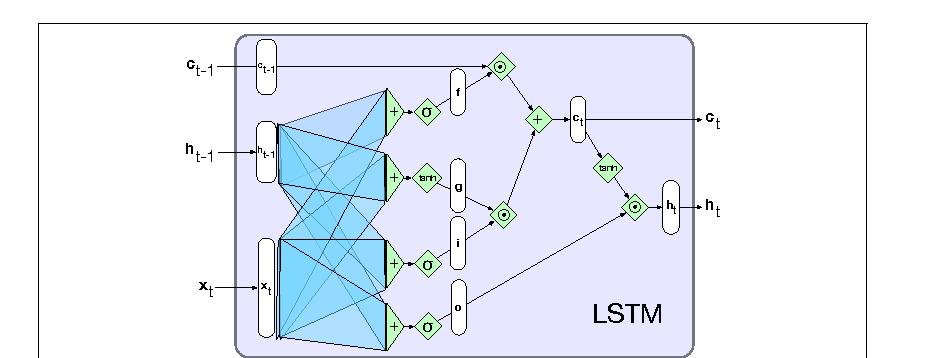
\includegraphics[width=0.90\linewidth]{J14_13}
  \end{center}
  \vspace{-0.4em}
  {\tiny\color{mcMuted}
  A single LSTM unit as a computation graph. The inputs are the current
  input $\mathbf{x}_t$, the previous hidden state $\mathbf{h}_{t-1}$ and the
  previous context $\mathbf{c}_{t-1}$; the outputs are the new hidden state
  $\mathbf{h}_t$ and the updated context $\mathbf{c}_t$. The top line is the
  context: multiplied by the forget gate, added to, and passed on, with
  no weight matrix on the path.
  \hfill Jurafsky \& Martin (2026), Fig.~14.13.\par}
\end{frame}

\begin{frame}{The LSTM cell, as a block diagram}
  \begin{columns}[T, onlytextwidth]
    \begin{column}{0.46\textwidth}
      \begin{center}
        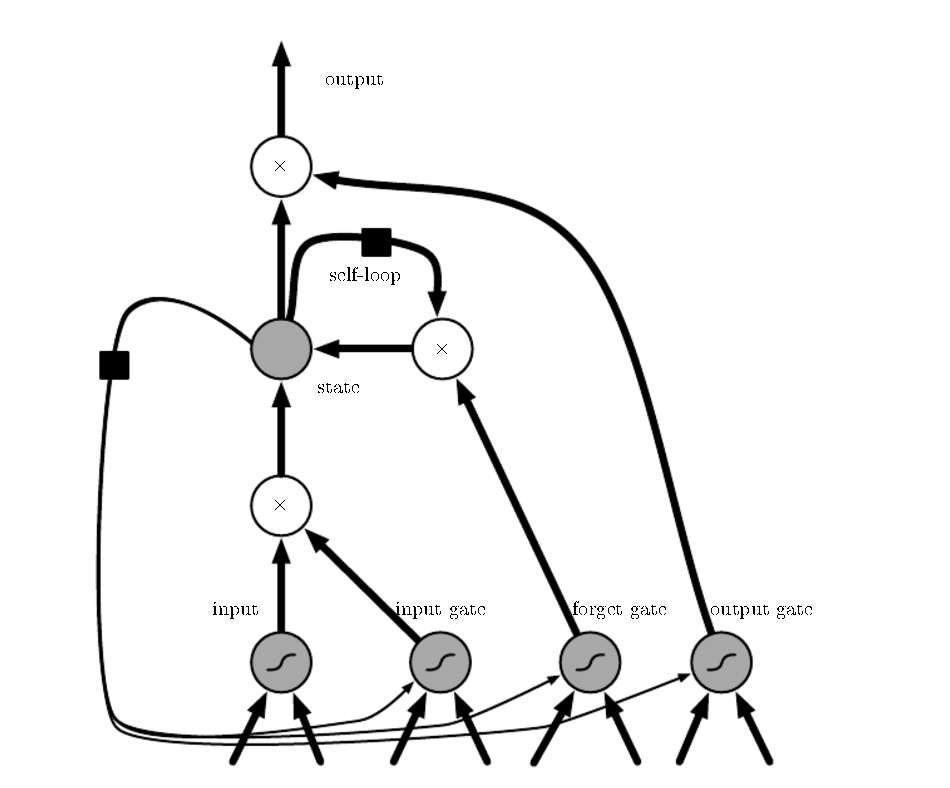
\includegraphics[width=0.98\linewidth]{G10_16}
      \end{center}
    \end{column}
    \begin{column}{0.52\textwidth}
      \vspace{0.2em}
      {\footnotesize
      \begin{itemize}\itemsep0.2em
        \item Goodfellow's drawing of the same cell: the state unit has
              a \alert{linear self-loop} whose weight is set by the
              forget gate
        \item An input feature, computed by an ordinary unit, is
              accumulated into the state if the input gate allows it
        \item The output can be shut off by the output gate; every gate
              is a sigmoid, the input unit any squashing nonlinearity
      \end{itemize}}
    \end{column}
  \end{columns}
  \vspace{-0.2em}
  {\tiny\color{mcMuted} Block diagram of the LSTM cell; cells replace
  the hidden units of an ordinary recurrent network.
  \hfill Goodfellow et al.\ (2016), \S10.10.1, Fig.~10.16.\par}
\end{frame}

\begin{frame}{Why the cell remembers}
  \vspace{-0.45em}
  \begin{propx}[The cell's gradient is a product of forget gates]\label{th:carousel}
    \small
    Holding the gates fixed, along the cell's own path
    $\ \partial\mathbf{c}_t/\partial\mathbf{c}_k = \prod_{s=k+1}^{t} \mathrm{diag}(\mathbf{f}_s)$,
    a product of numbers in $(0, 1)$ with \emph{no weight matrix and no
    activation derivative} in it: with $\mathbf{f}_s \approx \mathbf{1}$ the
    gradient passes unattenuated.
  \end{propx}
  \vspace{-0.15em}
  {\footnotesize
  \begin{itemize}\itemsep0.12em
    \item \focus{1}{Proof. $\mathbf{c}_s = \mathbf{f}_s \odot \mathbf{c}_{s-1} + \mathbf{j}_s$
          is linear in $\mathbf{c}_{s-1}$ with coefficient $\mathbf{f}_s$;
          chain the steps. \hfill $\square$}
    \item \focus{2}{Against Proposition~\ref{th:bound}: the simple
          cell's factor $\mathrm{diag}(g')\,\mathbf{U}$ is typically well
          below one; the LSTM's is a gate the network can hold at one
          --- the \alert{constant error carousel}. The gates depend on
          $\mathbf{h}_{t-1}$ too, so there are other paths; this is the one
          that survives.}
  \end{itemize}}
  \vspace{-0.3em}
  \srcline{Hochreiter \& Schmidhuber (1997); Gers et al.\ (2000); Goodfellow et al.\ (2016), \S10.10.1.}
\end{frame}


\begin{frame}{Gated units are drop-in modules}
  \vspace{-0.2em}
  \begin{center}
    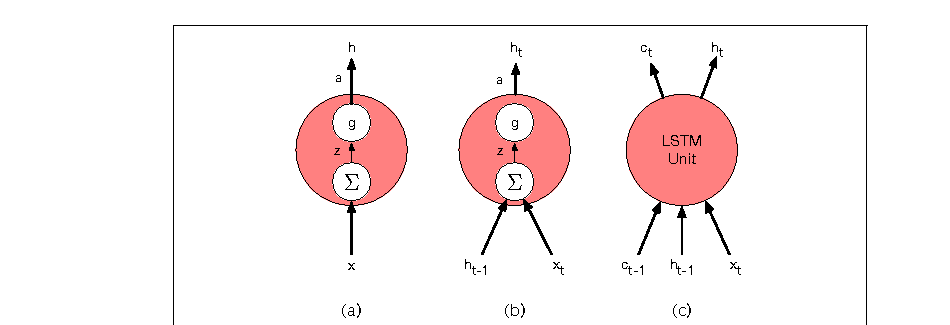
\includegraphics[height=0.40\textheight]{J14_14}
  \end{center}
  \vspace{-0.3em}
  {\footnotesize
  \begin{itemize}\itemsep0.16em
    \item (a) feedforward, (b) simple recurrent, (c) LSTM: the
          complexity is \alert{inside}; from outside, only the cell vector is new
    \item So an LSTM drops into every architecture of Classes 27 and
          29 and is unrolled and trained the same way
  \end{itemize}}
  \vspace{-0.3em}
  \srcline{Jurafsky \& Martin (2026), \S14.5.1, Fig.~14.14.}
\end{frame}

% =====================================================================
\section{Other Gated Cells}
% =====================================================================

\begin{frame}{The gated recurrent unit}
  \vspace{-0.3em}
  \begin{defx}[GRU]\label{th:gru}
    \small
    One gate decides both what to forget and what to write:
    \[
      \begin{aligned}
        \mathbf{u}_t &= \sigma(\mathbf{U}_u\mathbf{h}_{t-1} + \mathbf{W}_u\mathbf{x}_t) &&\text{update gate}\\
        \mathbf{r}_t &= \sigma(\mathbf{U}_r\mathbf{h}_{t-1} + \mathbf{W}_r\mathbf{x}_t) &&\text{reset gate}\\
        \tilde{\mathbf{h}}_t &= \tanh\big(\mathbf{U}_h(\mathbf{r}_t \odot \mathbf{h}_{t-1}) + \mathbf{W}_h\mathbf{x}_t\big) &&\text{candidate}\\
        \mathbf{h}_t &= \mathbf{u}_t \odot \mathbf{h}_{t-1} + (\mathbf{1} - \mathbf{u}_t) \odot \tilde{\mathbf{h}}_t &&\text{new state}
      \end{aligned}
    \]
  \end{defx}
  \vspace{-0.15em}
  {\footnotesize
  \begin{itemize}\itemsep0.12em
    \item No separate cell, three weight pairs against four. The update
          gate is a conditional leaky integrator per dimension; the reset
          gate chooses what of the past the candidate may see
  \end{itemize}}
  \vspace{-0.3em}
  \srcline{Goodfellow et al.\ (2016), Eqs.~10.45--10.47; Cho et al.\ (2014); Chung et al.\ (2014).}
\end{frame}

\begin{frame}{The GRU's state stays between old and new}
  \vspace{-0.3em}
  \begin{propx}[Convex update]\label{th:convex}
    \small
    Since every entry of $\mathbf{u}_t$ lies in $(0, 1)$, each coordinate of
    $\mathbf{h}_t = \mathbf{u}_t \odot \mathbf{h}_{t-1} + (\mathbf{1} - \mathbf{u}_t) \odot \tilde{\mathbf{h}}_t$
    lies between the old state and the candidate. Along the old state the
    derivative is $\mathrm{diag}(\mathbf{u}_t)$, so a coordinate with
    $u \approx 1$ is copied unchanged and its gradient passes unchanged,
    exactly as on the LSTM's cell line.
  \end{propx}
  \vspace{0.1em}
  {\footnotesize
  \begin{itemize}\itemsep0.24em
    \item \focus{1}{Proof. $u\,a + (1-u)\,b$ with $u \in (0, 1)$ is a
          convex combination of $a$ and $b$; differentiate in $a$.
          \hfill $\square$}
    \item \focus{2}{Which pieces of the LSTM are needed? Ablations
          find no variant that beats both LSTM and GRU across tasks;
          the forget gate is the crucial ingredient, and a forget bias of
          $1$ makes the LSTM as strong as the best variant.}
  \end{itemize}}
  \srcline{Goodfellow et al.\ (2016), \S10.10.2; Greff et al.\ (2017); Jozefowicz et al.\ (2015).}
\end{frame}


% =====================================================================
\section{Optimising Through Time}
% =====================================================================

\begin{frame}{Clipping the gradient}
  \vspace{-0.45em}
  \begin{propx}[Norm clipping keeps the direction]\label{th:clip}
    \small
    Replace the gradient $\mathbf{g}$ by
    \[
      \mathbf{g} \leftarrow \frac{\mathbf{g}\,v}{\|\mathbf{g}\|} \quad \text{if } \|\mathbf{g}\| > v .
    \]
    The step is still along $\mathbf{g}$, a descent direction, and its
    length is at most $\eta v$ whatever the gradient's size.
  \end{propx}
  \vspace{0.05em}
  {\footnotesize
  \begin{itemize}\itemsep0.2em
    \item \focus{1}{Proof. A positive scaling changes length only, and
          $\|\eta\mathbf{g}v/\|\mathbf{g}\|\| = \eta v$. \hfill $\square$}
    \item \focus{2}{Why: the loss over many steps has \alert{cliffs},
          flat regions separated by walls exponentially steep in the
          number of steps, since $\mathbf{U}$ multiplies itself once per
          step; one step at a cliff can undo all the descent so far.
          Clipping addresses explosion only.}
  \end{itemize}}
  \vspace{-0.3em}
  \srcline{Goodfellow et al.\ (2016), \S10.11.1, Eqs.~10.48--10.49; Pascanu et al.\ (2013); Mikolov (2012).}
\end{frame}

\begin{frame}{Clipping at a cliff, drawn}
  \begin{center}
    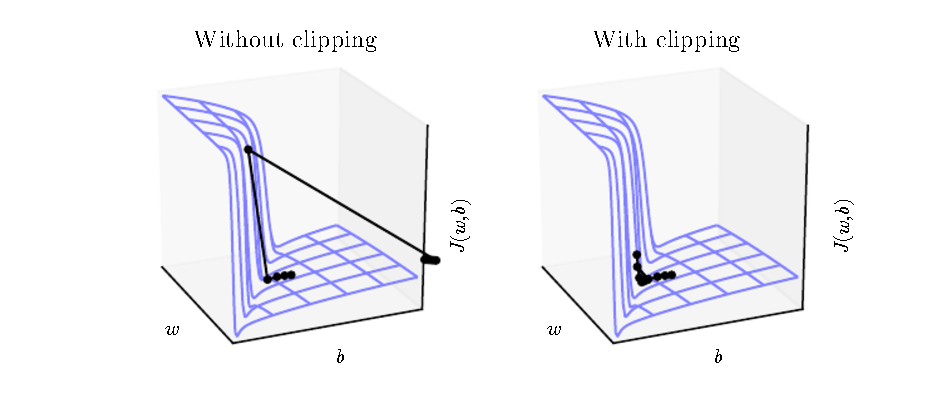
\includegraphics[width=0.82\linewidth]{G10_17}
  \end{center}
  \vspace{-0.5em}
  {\tiny\color{mcMuted}
  Gradient clipping in a recurrent network with two parameters $w$ and
  $b$. The cliff is exponentially steep in the number of time steps,
  because the weight matrix is multiplied by itself once per step.
  (Left) without clipping, descent overshoots the ravine and a very
  large gradient throws the parameters far away. (Right) with the norm
  clipped, the reaction is moderate and the descent stays in the ravine.
  \hfill Goodfellow et al.\ (2016), Fig.~10.17, after Pascanu et al.\ (2013).\par}
\end{frame}

\begin{frame}{Encouraging the gradient to flow}
  \vspace{0.05em}
  {\footnotesize
  \begin{itemize}\itemsep0.30em
    \item Clipping handles explosion; vanishing needs a path whose
          product of derivatives is near one --- the gates --- or a
          \alert{regulariser} that asks for it
    \item Pascanu et al.\ penalise, at every step, how much the
          back-propagated gradient shrinks in crossing that step:
          \[
            \Omega = \sum_t \left(
              \frac{\big\| (\nabla_{\mathbf{h}_t}L)^{\mathsf T}\,\partial\mathbf{h}_t/\partial\mathbf{h}_{t-1} \big\|}
                   {\|\nabla_{\mathbf{h}_t}L\|} - 1 \right)^2 ,
          \]
          treating $\nabla_{\mathbf{h}_t}L$ as a constant for the purpose
          of the regulariser
    \item With clipping alongside it, this lengthens the dependencies a
          simple RNN can learn; with abundant data it is not as
          effective as an LSTM, which is why the gate won
  \end{itemize}}
  \srcline{Goodfellow et al.\ (2016), \S10.11.2, Eqs.~10.50--10.52; Pascanu et al.\ (2013).}
\end{frame}

\begin{frame}{Where the gate leads: explicit memory}
  \vspace{-0.2em}
  \begin{columns}[T, onlytextwidth]
    \begin{column}{0.46\textwidth}
      \vspace{0.3em}
      {\footnotesize
      \begin{itemize}\itemsep0.2em
        \item The LSTM cell is a memory of one vector with learned
              write and read gates; a \alert{memory network} is a set of
              such cells, addressed by content
        \item A task network writes and reads through soft attention
              over the cells --- Class 27's softmax-weighted average
        \item Reading is differentiable, so it trains end to end; a
              fact is stored in one write, not many gradient steps
      \end{itemize}}
    \end{column}
    \begin{column}{0.52\textwidth}
      \begin{center}
        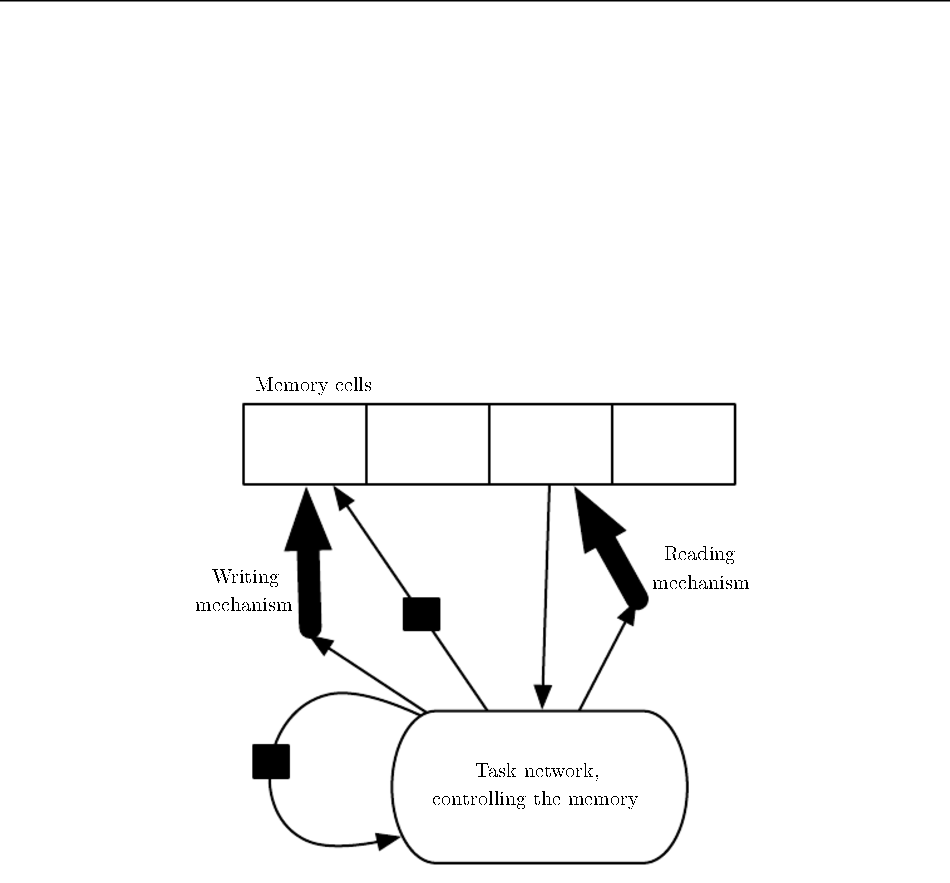
\includegraphics[width=0.66\linewidth]{G10_18}
      \end{center}
      \vspace{-0.3em}
      {\tiny\color{mcMuted} A network with an explicit memory: the task
      network controls the writing and reading mechanisms.
      Goodfellow et al.\ (2016), Fig.~10.18.\par}
    \end{column}
  \end{columns}
  \srcline{Goodfellow et al.\ (2016), \S10.12; Weston et al.\ (2014); Graves et al.\ (2014).}
\end{frame}

% =====================================================================
\section{Putting It Together}
% =====================================================================

\begin{frame}{The cell, opened}
  \vspace{0.2em}
  {\scriptsize
  \renewcommand{\arraystretch}{1.36}
  \begin{tabular}{@{}l@{\hspace{1.0em}}l@{\hspace{1.0em}}l@{\hspace{1.0em}}l@{}}
    & \textbf{state} & \textbf{path across time} & \textbf{derivative along it}\\
    simple RNN & $\mathbf{h}_t$ & through $\mathbf{U}$ and $g$ every step & $\mathrm{diag}(g')\,\mathbf{U}$, shrinks or explodes\\
    leaky unit & $\mu_t$ & a linear self-connection & the constant $\alpha$\\
    LSTM & $\mathbf{h}_t$ and $\mathbf{c}_t$ & the cell line & $\mathrm{diag}(\mathbf{f}_t)$, chosen by the network\\
    GRU & $\mathbf{h}_t$ & the update gate's copy & $\mathrm{diag}(\mathbf{u}_t)$, chosen by the network\\
  \end{tabular}}
  \vspace{0.6em}

  \begin{redhighlight}
    Every fix is the same fix: give the gradient a path whose factors
    stay near one. The gate is the version where the network decides,
    at every step, which facts get that path.
  \end{redhighlight}
\end{frame}

\begin{frame}{Takeaways}
  \vspace{-0.1em}
  {\scriptsize
  \begin{enumerate}\itemsep0.24em
    \item A repeated linear map raises its eigenvalues to the power of
          the time: components decay or explode geometrically
          (Theorem~\ref{th:power}), and the same product bounds the
          gradient of the nonlinear cell (Proposition~\ref{th:bound})
    \item A linear self-connection of weight near one is a running
          average with a long time constant, and a path the gradient
          survives (Proposition~\ref{th:leaky})
    \item The LSTM splits the state into a cell and a hidden vector,
          and manages the cell with three gates (Definition~\ref{th:lstm});
          along the cell line the gradient is a product of forget gates,
          with no weight matrix in it (Proposition~\ref{th:carousel})
    \item The GRU does the same with two gates and no separate cell;
          its update is a convex combination (Definition~\ref{th:gru},
          Proposition~\ref{th:convex})
    \item In practice the gated cells learn dependencies across many
          more steps than the simple RNN, which is why they are the
          default recurrent unit
    \item Norm clipping bounds the step without changing its direction
          (Proposition~\ref{th:clip}); an LSTM is a better answer to
          vanishing than any regulariser
  \end{enumerate}}
  \vspace{-0.2em}
  \bridge{Class 29 puts the cell to work: language models, taggers,
  classifiers, and what stacking and bidirectionality buy.}
\end{frame}

\begin{frame}[allowframebreaks]{References}
  \vspace{0.3em}
  {\scriptsize
  \begin{enumerate}\itemsep0.30em
    \item D.\ Jurafsky \& J.\ H.\ Martin, \emph{Speech and Language
          Processing}, 3rd ed.\ draft, August 2026. Ch.~14 \S14.5
          (Eqs.~14.20--14.27, Figs.~14.13--14.14), \S14.5.1.
    \item I.\ Goodfellow, Y.\ Bengio \& A.\ Courville, \emph{Deep
          Learning}, MIT Press, 2016. \S10.7 (Eqs.~10.36--10.39,
          Fig.~10.15), \S10.8, \S10.9, \S10.10 (Eqs.~10.40--10.47,
          Fig.~10.16), \S10.11 (Eqs.~10.48--10.52, Fig.~10.17),
          \S10.12 (Fig.~10.18).
    \item S.\ Hochreiter \& J.\ Schmidhuber, ``Long short-term memory'',
          \emph{Neural Computation} 9(8), 1997.
    \item F.\ A.\ Gers, J.\ Schmidhuber \& F.\ Cummins, ``Learning to
          forget: continual prediction with LSTM'', \emph{Neural
          Computation} 12(10), 2000.
    \item Y.\ Bengio, P.\ Simard \& P.\ Frasconi, ``Learning long-term
          dependencies with gradient descent is difficult'', \emph{IEEE
          Trans.\ Neural Networks} 5(2), 1994.
    \item R.\ Pascanu, T.\ Mikolov \& Y.\ Bengio, ``On the difficulty of
          training recurrent neural networks'', ICML 2013.
    \item K.\ Cho et al., ``Learning phrase representations using RNN
          encoder--decoder for statistical machine translation'',
          EMNLP 2014; J.\ Chung et al., ``Empirical evaluation of gated
          recurrent neural networks on sequence modeling'', 2014.
    \item K.\ Greff et al., ``LSTM: a search space odyssey'', \emph{IEEE
          TNNLS} 28(10), 2017; R.\ Jozefowicz, W.\ Zaremba \&
          I.\ Sutskever, ``An empirical exploration of recurrent network
          architectures'', ICML 2015.
    \item M.\ C.\ Mozer, ``Induction of multiscale temporal structure'',
          NeurIPS 1992; T.\ Lin et al., ``Learning long-term dependencies
          in NARX recurrent neural networks'', \emph{IEEE Trans.\ Neural
          Networks} 7(6), 1996.
    \item H.\ Jaeger \& H.\ Haas, ``Harnessing nonlinearity: predicting
          chaotic systems and saving energy in wireless communication'',
          \emph{Science} 304, 2004.
    \item T.\ Mikolov, \emph{Statistical Language Models Based on Neural
          Networks}, PhD thesis, Brno University of Technology, 2012.
    \item J.\ Weston, S.\ Chopra \& A.\ Bordes, ``Memory networks'',
          ICLR 2015 (arXiv 2014); A.\ Graves, G.\ Wayne \& I.\ Danihelka,
          ``Neural Turing machines'', arXiv:1410.5401, 2014.
  \end{enumerate}}
\end{frame}

\begin{frame}[standout]
  Questions?
\end{frame}

\end{document}
